% *****************************************************************************
% * Copyright (c) 2007 by Elexis
% * All rights reserved. This document and the accompanying materials
% * are made available under the terms of the Eclipse Public License v1.0
% * which accompanies this distribution, and is available at
% * http://www.eclipse.org/legal/epl-v10.html
% *
% * Contributors:
% *    G. Weirich - initial implementation
% *
% *  $Id: settings.tex 6282 2010-04-19 19:24:51Z niklausgiger $
% *******************************************************************************
%
% !Mode:: "TeX:UTF-8" (encoding info for WinEdt)

\label{settings}
Die Einstellungen sind alle im selben Dialog zusammengefasst, welcher unter
\textsc{Datei-Einstellungen} erreicht werden kann (Abb. \ref{fig:settingsmain}).
%\usepackage{graphics} is needed for \includegraphics
\begin{figure}[h]
\begin{center}
  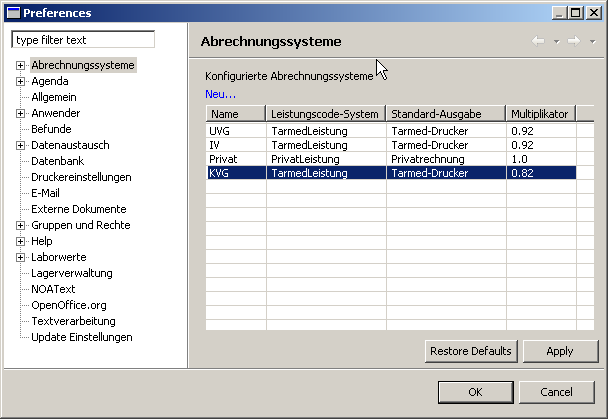
\includegraphics[width=0.6\textwidth]{images/settingsmain}
  \caption{Einstellungs-Dialog}
  \label{fig:settingsmain}
\end{center}
\end{figure}


Wie üblich in Elexis ist der genaue Inhalt dieses Dialogs davon abhängig,
welche Plugins installiert sind. Mit den Reitern auf der linken Seite wählt man
einen Bereich aus, für den man Einstellungen ändern möchte. Wir gehen hier auf
diejenigen Seiten ein, die zur Grundausstattung von Elexis gehören. Grundsätzlich
sollten alle Einstellungen \glqq Ab Werk\grqq{}vernünftige Grundeinstellungen
aufweisen, so dass es zunächst nicht nötig ist, hier etwas zu ändern. Sie
brauchen daher dieses Kapitel auch nicht unbedingt weiterzulesen.

\section{Abrechnungssysteme}
\label{settings:abrechnungssystem}
\index{Abrechnungssystem}
\index{KVG}\index{UVG}\index{TarMed}
Auf dieser Seite legen Sie fest, welche Arten von Abrechnungssystemen in Ihrer Praxis verwendet werden.

Da Elexis ein universelles Programm ist, welches nicht nur Ärzte, sondern auch Angehörige anderer Gesundheitsberufe unterstützen kann, ist das Abrechnungssystem sehr offen und gehalten. Das bedeutet, dass anfänglich eine entsprechende Konfiguration notwendig ist.

Die Verrechnung von Leistungen hat drei grundsätzliche Elemente:
\begin{enumerate}
    \item Ein Codesystem, also vereinfacht gesagt ein Konzept, um einzelne Leistungen und deren Wert zu benennen. Beispiel: \glqq Tarmed\grqq{}, \glqq Akupunkturtarif\grqq{} usw.
   \item Ein Garantenkonzept, also wer bekommt die Rechnung, wer bezahlt letztlich usw. Beispiele: Tiers Garant, Privatrechnung etc.
   \item Ein Rechnungskonzept: Wie muss die Rechnung aussehen, auf welchem Weg wird sie versandt (elektronisch, Papier)
\end{enumerate}

Eine Kombination aus Codesystem,Garantenkonzept und Rechnungskonzept nennen wir hier \glqq Abrechnungssystem\grqq{}.

Man kann in Elexis beliebig viele Abrechnungssysteme definieren, welche parallel existieren und je nach Bedarf verwendet werden können.

Jedes Abrechnungssystem hat bestimmte Eigenschaften:\\
\begin{wrapfigure}{l}{5cm}
    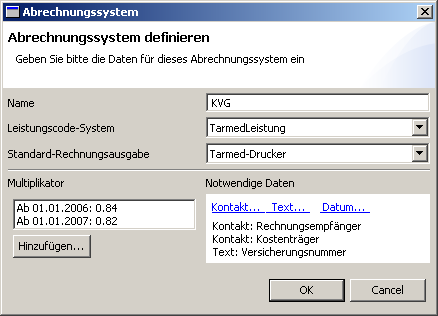
\includegraphics[width=4.7cm]{images/abrechnungssystem1}
    \caption{Abrechnungssystem Detail}
    \label{fig:abr1}
\end{wrapfigure}

Der Name ist frei wählbar, Leistungscode-System und Standard-Rechnungsausgabe können aus den installierten Plugins gewählt werden (Für nicht vorhandene Abrechnungssysteme müssten entsprechende Plugins erstellt werden).
Der Multiplikator ist ein Faktor, der auf jede einzelne Position angewendet wird, wenn sie verrechnet wird. Man kann also verschiedene Abrechnungssysteme mit demselbem Leistungscode-System, aber verschiedenen Multiplikatoren (\glqq Taxpunkten\grqq{}) haben. Mit \textit{Hinzufügen} kann man einen Multiplikator definieren, welcher immer ab einem bestimmten Datum gilt.

Und schliesslich sind je nach Abrechnungssystem bestimmte Angaben notwendig, um die Leistungen zu verrechnen, beispielsweise Rechnungsempfänger, Kostenträger, Nummern etc.
Elexis macht hier keine Vorschriften, Sie können eingeben, was immer Sie wollen. Es sind die Datentypen Text, Kontakt und Datum möglich. (Bei UVG-Versicherungen beispielsweise auch \glqq Unfalldatum\grqq{}).\\


\section{Allgemein}
Auf dieser Seite werden allgemeine Einstellungen für den Programmablauf
definiert. Es sind dies:
\subsection{Einstellungen zum Log}
Das \glqq Log\grqq{} ist das Logbuch eines Programmes. Hier werden verschiedene
Information zum Programmablauf gespeichert, welche z.B. bei der Fehlersuche
nützlich sein können.
\begin{itemize}
  \item Logdatei: Der Ort, an den die Log-Informationen gespeichert werden. Dies sollte normalerweise eine Datei \glqq elexis.log\grqq{} in Ihrem
  Datenverzeichnis sein. Der Wert \glqq none\grqq{} ist nur sinnvoll, wenn Sie
  Elexis aus einer Entwicklungsumgebung heraus starten.
  \item Log-Stufe: Wieviele Meldungen ausgegeben werden sollen. Auf Stufe 1
  werden nur die allerschlimmsten Fehler, die einen Programmabbruch erzwingen,
  ausgegeben. Auf Stufe 5 werden sehr viele Meldungen, die nur in speziellenj
  Fällen sinnvoll sind, ins Log geschrieben. Wir empfehlen für den Normalbetrieb
  Stufe 2 oder 3.
  \item Alert-Stufe: Meldungen, die den entsprechenden Schweregrad haben, werden
  nicht nur ins Log geschrieben, sondern gleich am Bildschirm angezeigt.
  Achtung: Wenn Sie hier eine zu hohe Stufe angeben, werden Sie ständig durch
  aufpoppende Meldungsboxen irritiert werden. Wir empfehlen Stufe 1.
  \item Tabellenname für Trace: Trace bedeutet, dass alle Aktionen in einer
  speziellen Tabelle aufgezeichnet werden. Es lässt sich damit später
  nachvollziehen, von welcher Arbeitsstation aus zu welchem Zeitpunkt welche
  Aktion mit Elexis durchgeführt wurde. Dies erlaubt eine sehr genaue Kontrolle
  der Vorgänge, kostet aber natürlich Arbeitsgeschwindigkeit und Speicherplatz.
  Wir empfehlen im Normalfall die Einstellung \glqq none\grqq{}.
  \item Bevorzugte Sprache: Diese Einstellung definiert nicht, welche
  Sprachversion von Elexis ausgeführt wird (Das wird anhand der
  Betriebssystemeinstellungen und ggf. Startparameter entschieden), sondern
  vielmehr, welche Tarmed- und ICD-Versionen etc. importiert werden.
  \item Speicherdauer im Cache: Dies ist eine sehr technische Einstellung. Es
  geht darum, wie lange aus der Datenbank gelesene Objekte gültig bleiben
  sollen, bevor sie erneut gelesen werden. Wenn
  viele Arbeitsstationen im Netz sind, geben Sie hier besser kürzere Zeiten an
  (z.B. 5 Sekunden), wenn Sie von zuhause über eine langsame Internet-Verbindung
  auf Elexis zugreifen, eher eine längere Zeit (z.B. 300 Sekunden).
  \item Aktualisierungsintervall: Nach welcher Zeitspanne soll Elexis jeweils
  seine Views aktualisieren. Wenn beispielsweise die MPA einen Patienten der
  Agenda auf \glqq eingetroffen\grqq{} setzt, dann dauert es maximal soviele
  Sekunden, bis diese Statusänderung auf Ihrem Bildschirm sichtbar ist. Wenn Sie
  zu kurze Zeiten angeben, wird die Netzwerkbelastung unnötig hoch.
\end{itemize}
\section{Anwender}
In diesem Zweig der Einstellungen sind anwenderspezifische Einstellungen
untergebracht. Wenn Sie einheitliche Einstellungen möchten, können Sie auch einen
Einstellungssatz unter einem frei wählbaren Namen speichern und von einem
anderen Anwenderaccount oder Abreitsstation aus wieder unter diesem Namen laden.

Die Buttons \glqq Einstellungen laden von\ldots\grqq{} bzw. \glqq Einstellungen
speichern nach\ldots\grqq{} betreffen hierbei die anwenderspetifischen
Einstellungen(im Wesentlichen alles was im Zweig \textsc{Anwender} der
Einstellungen vorhanden ist), während die Buttons \glqq
Arbeitsplatzeinstellungen \ldots\grqq{} die auf der lokalen Station
gespeicherten Perspektivenlayouts betreffen.
\subsection{Anwender - Ansicht}
\label{userconfig}
Hier sind verschiedene Ansichtsoptionen zusammengefasst:
\begin{itemize}
\item Erweiterbare Felder: Hier geht es um die 'aufklappbaren' Felder in manchen Views, z.B. der Patient-Detail View die Felder Diagnosen oder Bemerkungen etc. Man kann festlegen, dass solche Felder immer erstmal geschlosse oder immer erstmal geöffnet sein sollen, oder dass sie sich ihren letzten Zustand merken sollen.
\item Anzuzeigende Felder in Patientenliste: Dies definiert die Filterfelder mit denen man in der Patientenliste Patienten suchen kann. Standardmässig werden Name, Vorname und Geburtsdatum als Filterkriterien angeboten, man kann aber auch PatientNr anzeigen lassen.

\item Zusatzfelder im Patient-Detail-Blatt: Hier können Sie beliebige zuätzliche Text-Angaben erfassen, die Sie für einen Patienten erfassen können wollen, und die nicht mit Bemerkungen oder Etiketten erfasst werden können. Geben Sie einfach pro Zeile einen Namen für einen abzuspeichernden Datentyp ein.

\end{itemize}

\subsection{Anwender - Schriftarten}
Hier können Sie die Standardschriftart und -grösse für alle View-Inhalte angeben. Einzelne Views und Plugins können immer noch andere Schriftarten einstellen, aber dies ist die Standardvorgabe.

\section{Datenaustausch}
Dies ist eine Sammelkategorie für Einstellungen von Plugins, die Datenaustausch von und nach Elexis anbieten. Ob und welche Einstellungsseiten hier zu finden sind, hängt von den installierten Transport-Plugins ab.
\section{Datenbank}
Anzeige von Einstellungsdetails der aktuellen Datenbankverbindung
\section{Druckereinstellungen}
Hier kann man für jede Papierart den dazugehörigen Drucker und -Schacht auswählen. Beim Labeldrucker kann man ausserdem einstellen, ob der Druckerauswahldiealog überhaupt jedesmal vor dem Drucken angezeigt werden soll (wenn man z.B. mehrere Labeldrucker hat).
\section{E-Mail}
Diese Einstellungen sind für das Versenden von E-Mails aus Elexis wichtig. Dies wird inbesondere beim automatischen Versenden von Fehlermeldungen verwendet. 

\section{Gruppen und Rechte}
Dies ist die zentrale Benutzerverwaltung. Auf diesen Einstellungsseiten können Anwender und Mandanten eingerichtet und die Zugriffsrechte verteilt werden. Das Konzept der Gruppen ist auf Seite \pageref{sec:gruppen} genauer erläutert.
Legen Sie zunächst unter \textsc{Gruppen und Rechte} fest, welche Anwendergruppen Sie benötigen.
Um einen neuen Anwender oder Mandanten einzurichten, müssen Sie diesen zunächst als \glqq Kontakt \grqq{} erfassen, und dort unter Kontakt-Details als Anwender bzw. Mandant kennzeichnen. Dann können Sie unter \textsc{Gruppen und Rechte - Mandanten} dem Mandanten einen Benutzernamen und ein Passwort zuordnen, und angeben, welchen Gruppen er zugehörig sein soll.
Unter \textsc{Gruppen und Rechte - Anwender} können Sie dasselbe für Anwender angeben, ausserdem noch, für welchen Mandant dieser Anwender normalerweise tätig ist.
Unter \textsc{Gruppen und Rechte - Zugriffsteuerung} können für jede Gruppe und jeden Anwender einzeln Rechte zugeordnet werden.  (S. \ref{sec:gruppen}).
\section{Laborwerte}
\label{config:labor}
Hier können die in der Praxis benötigten Laborparameter definiert werden. Dies kann manuell geschehen, oder, bei Laborimport-Plugins können Laboritems auch automatisch mit den vom Labor gelieferten Angaben erstellt werden.
Jedes Laboritems ist durch folgende Eckdaten gekennzeichnet:
\begin{itemize}
\item{Einen Namen}
\item{Ein Kürzel}
\item{Das Labor, von dem es stammt}
\item{Den Normbereich, gegeben durch die Methode, z.T. auch geschlechts- alters- zyklusabhängig}
\item{Eine Gruppe, unter der des aufgelistet wird (z.B. Hämatologie)}
\item{Eine Sequenznummer, die angibt, an welcher Stelle innerhalb der Gruppe es einsortiert wird.}
\item{einen Typ (numerisch, absolut, text, Formel)}
\end{itemize}

Jedes Laborresultat ist durch ein solches Item, ein Datum und einen Patienten eindeutig identifiziert.
Es kann deswegen durchaus mehrere Items für ein- und denselben Parameter geben. Beispielsweise kann es ein Item \textsc{Vitamin B12} von verschiedenen Labors geben, welche nicht zwingend denselben Normbereich haben müssen.
Sie können die Liste der Tabelle durch Klick auf die Spaltenköpfe umsortieren.

Mit \textsc{Neuer Laborparameter} können Sie manuell ein neues Item erstellen\footnote{Beim Import von Laborwerten aus externen Labors werden die benötogten Items je nach Import-Plugin idR. automatisch erstellt.} und die oben genannten Angaben eingeben. Hier ist es sehr wichtig, dass Sie sich im Voraus genau überlegen, welche Laborparameter Sie benötigen, und wie Sie diese gruppiert haben wollen.
%\usepackage{graphics} is needed for \includegraphics
\begin{figure}[htp]
\begin{center}
  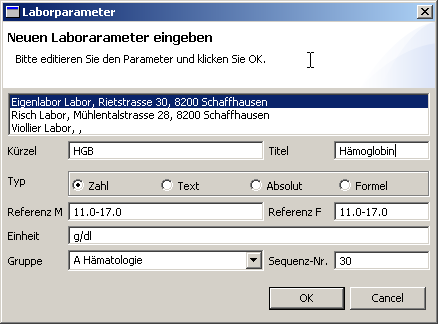
\includegraphics{images/labor1}
  \caption{Neues Labor-Item erstellen}
  \label{fig:labor1}
\end{center}
\end{figure}

In Abb. \ref{fig:labor1} sehen Sie den Dialog zum Anlegen eines neuen bzw. Ändern eines existierenden Items. Ganz oben geben Sie da Labor ein, von dem es stammt (Das Labor muss bereits als Kontakt erfasst sein). Kürzel und Titel sind die Anzeige des Items. Als Typ wählen Sie \textit{Zahl}, \textit{Text} (Für Parameter, die sich nicht als Zahl darstellen lassen, z.B. Bakteriologiebefunde), \textit{Absolut} für Parameter, die nur positiv oder negativ sein können und \textit{Formel} für Resultate, die errechnet werden sollen (z.B. LDL-Cholesterin gem. Friedewald- Dies ist weiter unten (\ref{ref:formel}) genauer erklärt).

Unter \textit{ReferenzM} geben Sie den Referenzbereich für Männer, unter \textit{ReferenzF} für Frauen ein \footnote{Elexis benötigt diese Angaben, um numerische Laborresultate automatisch als pathologisch darstellen zu können. Es ist deshalb wichtig, dass Sie den Referenzbereich genauso, als von-bis eingeben.}, unter \textit{Einheit} entsprechend die Masseinheit für den Parameter.

Unter \textit{Gruppe} geben Sie an, wo dieser Parameter gruppiert sein soll. Bereits existierende Gruppen sind in der Combobox schon enthalten und können einfach ausgewählt werden. Um eine neue Gruppe zu erstellen, können Sie den Namen einfach eintippen. Der Gruppenname muss folgendes Format haben:
Ein- oder mehrere Buchstaben, ein Leerzeichen, dann ein beliebiger Text. Die räfix entscheidet über die Sortierung auf dem Laborblatt. So wird die Gruppe  \textit{A Hämatologie} oberhalb von \textit{B Elektrolyte} zu stehen kommen, und \textit{DA Leberwerte} vor \textit{DC Nierenparameter}. Die Bennenung und die Reihenfolge der Gruppen bleibt ganz Ihnen überlassen.

Unter \textit{Sequenz-Nr} schliesslich geben Sie ein, wo innerhalb der Gruppe dieser Parameter auf dem Laborblatt stehen soll. Dies muss eine Zahl sein. Hierbei kommt es nicht auf den Abstand der Zahlen der einzelnen Items an, sondern nur auf die Grösse relativ zueinander. Es ist empfehlenswert, die Zahlen nicht unmittelbar aufeinanderfolgend zu wählen, damit man später ev. leicht noch etwas dazwischenfügen kann.

\subsection{Berechnete Laborwerte (Typ Formel)}
\label{ref:formel}
\index{Formel}
\index{Laborwert!formel}
Ein Laborparameter vom Typ \textit{Formel} wird nicht eingetragen oder eingelesen, sondern mit einer -im Prinzip beliebigen- Formel berechnet. In der Regel wird man sich dabei auf andere Laborwerte beziehen, von welchen der zu errechnende Parameter abhängig ist. Als Beispiel wollen wir hier einen Parameter für LDL, berechnet nach der Friedewald-Formel, erstellen. Diese Fromel benötigt als Parameter die Werte für Gesamtcholesterin, Triglyceride und HDL-Cholesterin, sie lautet ja: \textit{Gesamtcholesterin-HDL-(TG/2.2)}. Für user Beispiel seien diese anderen Parameter so vorhanden:
\begin{itemize}
  \item Gesamtcholesterin in Gruppe \textit{G Fettstoffwechsel}, Sequenznummer 10
  \item HDL-Cholesterin in Gruppe \textit{G Fettstoffwechsel}, Sequenznummer 20
  \item Triglyceride in Gruppe \textit{G Fettstoffwechsel}, Sequenznummer 40
\end{itemize}

Wir erstellen jetzt einen neuen Parameter namens \textit{LDL (errechnet)} in Gruppe G und geben ihm z.B. die Sequenznummer 21 (hier sehen Sie, dass es gut war, dass wir bei den vorherigen Sequenznummern Lücken gelassen haben) (Abb. \ref{fig:labor2}).
%\usepackage{graphics} is needed for \includegraphics
\begin{figure}[htp]
\begin{center}
  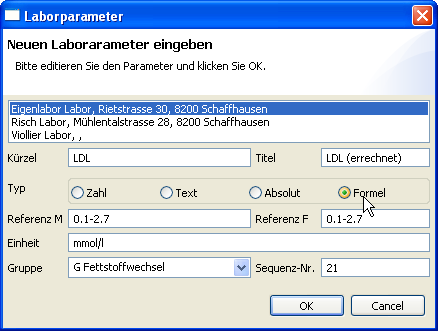
\includegraphics{images/labor2}
  \caption{Berechneten Laborwert erstellen}
  \label{fig:labor2}
\end{center}
\end{figure}
 Dann Klicken Sie bitte auf die Typbezeichnung \textit{Formel}. Es öffnet sich ein Eingabedialog zum Eingeben der Formel:\\
 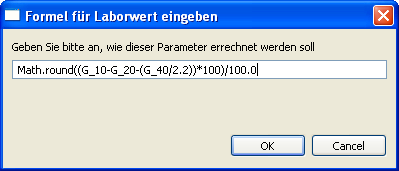
\includegraphics{images/labor3}\\
Um uns in der Formel auf andere Laborparameter zu beziehen, verwenden wir deren Gruppenindex (also das was vor dem Leerzeichen in der Gruppenbezeichnung steht) und Sequenznummer, getrennt durch einen Unterstrich. Um Gesamtcholesterin zu referenzieren, wählen wir also die Bezeichnung G\_20. Die Friedewald-Formel wird damit zu \textit{G\_10-G\_20-(G\_40/2.2)}. Dies würde dann allerdings auf 9 Stellen genau ausgegeben. Deshalb runden wir in unserem Beispiel mittels Math.round noch auf 2 Stellen.

 Wenn jetzt die Laborwerte, auf die sich die Formel bezieht, eingegeben werden, dann wird Elexis jeweils versuchen, die Formel auszuwerten. Wenn das nicht gelingt, weil beispielsweise noch nicht alle benötigten Parameter eingegeben sind, wird \textit{?formel?} eingesetzt (S. Abb.  \ref{fig:labor4}).
 %\usepackage{graphics} is needed for \includegraphics
\begin{figure}[htp]
\begin{center}
  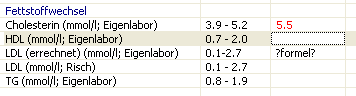
\includegraphics{images/labor4}
  \caption{Laboreintrag, noch nicht komplett}
  \label{fig:labor4}
\end{center}
\end{figure}

Erst wenn alle benötigten Parameter vorhanden sind, wird der errechnete Wert eingesetzt (Abb. \ref{fig:labor5}).
%\usepackage{graphics} is needed for \includegraphics
\begin{figure}[htp]
\begin{center}
  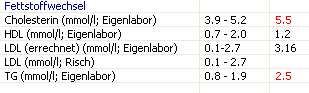
\includegraphics{images/labor5}
  \caption{Laboreintrag, komplettiert}
  \label{fig:labor5}
\end{center}
\end{figure}

\section{Leistungscodes}
Dies ist wieder eine Sammelrubrik, die je nach vorhandenen Plugins für die Leistungsabrechnung unterschiedlich gefüllt sein kann. In der Schweiz ist hier standardmässig Labortarif und Tarmed vorhanden. Diese sind auf Seite \pageref{arzttarife} genauer erklärt.

\section{Textverarbeitung}
Auch die verwendete Textverarbeitung für Briefe etc. ist in Elexis ja durch Plugins frei definierbar. Welche Textverarbeitung verwendet werden soll, kann hier eingestellt werden. Diese Einstellung sollte normalerweise nicht mehr verändert werden, wenn erste Dokumente erstellt wurden, da diese sonst eventuell nicht mehr ohne weiteres lesbar wären. Wir empfehlen, unter Windows das Plugin NOAText und unter Linux Office-Wrapper zu verwenden.
